%==================== API 2025 — Humming to Music Project ====================
% Compile with pdfLaTeX or XeLaTeX
%=============================================================================

\documentclass[11pt]{article}
\usepackage[margin=1in]{geometry}
\usepackage{graphicx}
\usepackage{float}
\usepackage{booktabs}
\usepackage{amsmath}
\usepackage{hyperref}
\usepackage{xcolor}
\usepackage{listings}
\usepackage{tikz}
\usetikzlibrary{shapes.geometric, arrows.meta, positioning, fit, backgrounds}

\hypersetup{colorlinks=true, linkcolor=black, urlcolor=blue, citecolor=blue}

% Code listing style
\lstset{
    language=Python,
    basicstyle=\ttfamily\small,
    keywordstyle=\color{blue},
    commentstyle=\color{gray},
    stringstyle=\color{red},
    numbers=left,
    numberstyle=\tiny\color{gray},
    frame=single,
    breaklines=true,
    captionpos=b
}

\title{From Humming to Soundtrack:\\Melody Extraction and Style-Transfer Music Generation}
\date{\today}
\author{Houhua Ma  4247477    Xijie Cao  4245016 \\Xiangyu Li  4386299        Xiaobin Tang 4221923\\}

\date{\today}

\begin{document}
\maketitle

\begin{abstract}
This report presents a prototype system that transforms raw humming or vocal recordings into polished, style-transferred musical tracks. The pipeline integrates classical audio signal processing techniques with modern generative modeling concepts, addressing challenges such as noise reduction, pitch extraction from unstable vocal input, melodic similarity preservation, and multi-style music generation. Our implementation demonstrates an end-to-end workflow from audio input through preprocessing, melody extraction, symbolic representation, conditional generation, and similarity evaluation. The system supports multiple musical styles including lofi, orchestral, 8-bit chiptune, rock, and ambient, enabling creative applications in game development, film scoring, and rapid music prototyping.
\end{abstract}

%=============================================================================
\section{Introduction}
%=============================================================================

Music creation has traditionally required specialized training and access to instruments or digital audio workstations. However, the most fundamental musical element---melody---can be expressed by anyone through humming or singing. This project addresses a compelling question: how can a simple hummed melody, captured on a smartphone in a noisy environment, be transformed into a polished musical soundtrack?

Consider a game developer who conceives a catchy tune while walking home. They record it on their phone, but the audio is rough, containing background noise, pitch instabilities, and no harmonic accompaniment. Our system bridges this gap by implementing a complete pipeline that processes such raw input and generates stylized musical output while preserving the original melodic intent. The project combines several audio processing and indexing concepts: signal-level processing handles noise reduction and normalization, pitch tracking algorithms extract the melodic contour, the extracted melody is converted into a symbolic representation suitable for music generation, and similarity metrics quantify how well the generated output preserves the original melodic characteristics.

The novelty of this work lies in combining audio processing and indexing techniques with music generation within a unified framework. By leveraging pre-trained pitch tracking algorithms and designing a modular architecture that can accommodate various generation backends, we create a practical workflow that bridges the gap between raw vocal input and polished musical output. This approach has immediate applications in creative industries where rapid melodic prototyping is valuable, such as indie game development, short film production, and music composition assistance.

%=============================================================================
\section{System Architecture}
%=============================================================================

The system follows a modular pipeline architecture where each component handles a specific transformation stage. This design philosophy allows independent development and testing of each module while maintaining clear data flow contracts between stages. As illustrated in Figure~\ref{fig:architecture}, the pipeline consists of nine interconnected modules that progressively transform raw audio into styled musical output.

\begin{figure}[H]
\centering
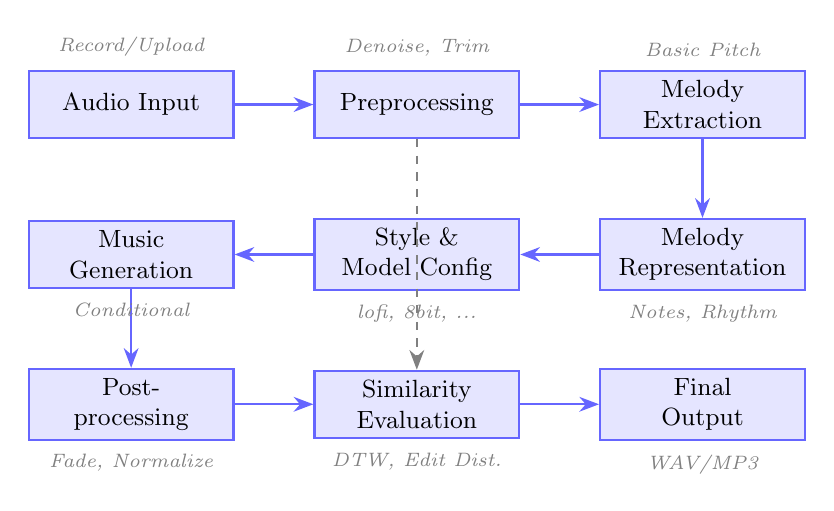
\begin{tikzpicture}[
    node distance=0.7cm and 1.0cm,
    box/.style={rectangle, draw=blue!60, fill=blue!10, thick, minimum width=2.6cm, minimum height=0.85cm, align=center, font=\small},
    arrow/.style={-{Stealth[length=2.5mm]}, thick, draw=blue!60},
    label/.style={font=\scriptsize\itshape, text=gray}
]

% Main pipeline boxes - row 1
\node[box] (input) {Audio Input};
\node[box, right=of input] (preprocess) {Preprocessing};
\node[box, right=of preprocess] (extract) {Melody\\Extraction};

% Row 2
\node[box, below=1.0cm of extract] (represent) {Melody\\Representation};
\node[box, left=of represent] (style) {Style \&\\Model Config};
\node[box, left=of style] (generate) {Music\\Generation};

% Row 3
\node[box, below=1.0cm of generate] (postprocess) {Post-\\processing};
\node[box, right=of postprocess] (similarity) {Similarity\\Evaluation};
\node[box, right=of similarity] (output) {Final\\Output};

% Arrows - row 1
\draw[arrow] (input) -- (preprocess);
\draw[arrow] (preprocess) -- (extract);

% Arrows - transition to row 2
\draw[arrow] (extract) -- (represent);
\draw[arrow] (represent) -- (style);
\draw[arrow] (style) -- (generate);

% Arrows - transition to row 3
\draw[arrow] (generate) -- (postprocess);
\draw[arrow] (postprocess) -- (similarity);
\draw[arrow] (similarity) -- (output);

% Dashed line for reference comparison
\draw[arrow, dashed, draw=gray] (preprocess.south) -- ++(0,-0.35) -| (similarity.north);

% Labels
\node[label, above=0.05cm of input] {Record/Upload};
\node[label, above=0.05cm of preprocess] {Denoise, Trim};
\node[label, above=0.05cm of extract] {Basic Pitch};
\node[label, below=0.05cm of represent] {Notes, Rhythm};
\node[label, below=0.05cm of style] {lofi, 8bit, ...};
\node[label, below=0.05cm of generate] {Conditional};
\node[label, below=0.05cm of postprocess] {Fade, Normalize};
\node[label, below=0.05cm of similarity] {DTW, Edit Dist.};
\node[label, below=0.05cm of output] {WAV/MP3};

\end{tikzpicture}
\caption{System architecture showing the nine-module pipeline. The dashed line indicates that the original preprocessed audio serves as reference for similarity evaluation against the generated output.}
\label{fig:architecture}
\end{figure}

The pipeline accepts audio input through either microphone recording or file upload, supporting common formats including WAV, MP3, M4A, FLAC, OGG, and AIFF. All audio is normalized to 16 kHz mono format for consistent downstream processing, with duration constraints between 0.5 and 30 seconds to ensure practical processing times while accommodating typical melodic phrases. The configuration system uses Python dataclasses to define parameters for each stage, enabling easy customization without code modifications.

%=============================================================================
\section{Methodology}
%=============================================================================

\textbf{Audio Input and Preprocessing.} The audio input module serves as the entry point for user-provided recordings, handling both real-time microphone capture and file uploads. When recording, the system uses the sounddevice library to capture audio at the configured sample rate with appropriate channel settings. For uploaded files, pydub provides format detection and conversion capabilities, automatically handling the diversity of audio formats users might provide. All input undergoes validation to ensure duration falls within acceptable bounds, rejecting clips that are too short to contain meaningful melodic content or too long for efficient processing.

The preprocessing stage addresses the inherent noisiness of casual vocal recordings through a sequence of signal conditioning operations. Silence trimming identifies and removes leading and trailing silent regions using energy-based detection, where the algorithm scans for segments exceeding a threshold of $-40$ dB for a minimum duration of 100 ms, retaining 50 ms padding around boundaries to preserve natural attack and release characteristics. A high-pass filter at 80 Hz removes low-frequency rumble and handling noise common in handheld recordings while preserving fundamental frequencies of typical singing ranges. Loudness normalization then ensures consistent input levels by calculating current RMS level and applying gain adjustment to reach $-20$ dB RMS, followed by peak normalization with 0.1 dB headroom to prevent clipping.

\textbf{Melody Extraction.} Extracting the fundamental frequency contour from vocal input presents significant challenges due to pitch instabilities, vibrato, breathiness, and the quasi-periodic nature of the human voice. Our implementation employs Basic Pitch, a neural network-based pitch detection model developed by Spotify, which leverages deep learning to achieve robust pitch tracking even in noisy conditions. Unlike traditional autocorrelation-based methods, Basic Pitch uses a lightweight convolutional neural network trained on diverse musical audio to predict pitch, onset, and note activations simultaneously. The model estimates pitch within the typical vocal range while providing polyphonic capability, though our pipeline focuses on monophonic melody extraction.

Post-processing refines the raw pitch estimates through median filtering with a 5-frame window, smoothing micro-variations and occasional tracking errors while preserving intentional pitch changes. The note confidence scores provided by Basic Pitch are thresholded to distinguish voiced from unvoiced regions, with segments shorter than 100 ms removed to eliminate spurious detections arising from transient noise or breath sounds. The output consists of synchronized arrays containing timestamps, F0 values in both Hertz and MIDI note numbers (facilitating musical interpretation), and binary voiced/unvoiced flags that indicate where actual melodic content exists.

\textbf{Melody Representation.} Converting the continuous pitch contour into discrete symbolic representation enables compatibility with music generation systems and provides compact melodic encoding. The note segmentation algorithm groups consecutive voiced frames into discrete note events, computing a stable pitch value for each segment using the median of frame-level estimates, which proves robust against momentary tracking fluctuations. Segments shorter than 120 ms are discarded as likely artifacts, while adjacent notes with similar pitches (within 0.35 semitones tolerance) separated by brief gaps are merged to handle natural variations in sustained tones.

The rhythm profile captures temporal characteristics through several derived features. Tempo estimation uses the median inter-onset interval between consecutive notes, providing a beats-per-minute approximation. A duration histogram categorizes note lengths into bins, revealing whether the melody consists primarily of short staccato notes or longer sustained tones. Quantized patterns discretize onset times and durations to 250 ms steps, producing grid-aligned representations suitable for rhythmic comparison. An optional seven-dimensional embedding vector summarizes statistical properties including pitch mean, standard deviation, range, duration statistics, and note count, supporting rapid similarity queries and potential melody retrieval applications.

\textbf{Style Configuration and Music Generation.} The style configuration module defines musical style presets that guide generation, with each preset encapsulating descriptive attributes including mood classification, target tempo, characteristic instruments, and model-specific text prompts. Five styles are currently implemented: lofi (relaxed hip-hop at 80 BPM with soft drums and warm textures), orchestral (cinematic at 110 BPM with strings and brass), 8-bit (playful chiptune at 130 BPM with square wave leads), rock (energetic at 120 BPM with guitars and punchy drums), and ambient (calm soundscapes at 70 BPM with evolving pads and drones).

The music generation module implements an adapter pattern that decouples the generation interface from specific model implementations, allowing seamless integration of different backends without modifying pipeline logic. The base adapter class defines a standard interface accepting melody representation, style preset, model configuration, and output parameters. The current prototype includes a stub generator that synthesizes a sine wave at the melody's average pitch, serving as a verification tool for data flow correctness. Production deployment would replace this with calls to pre-trained neural models such as MusicGen or Riffusion, where melody representation and style prompts would condition generation to produce full arrangements preserving the input melodic contour while adding appropriate harmonic accompaniment and timbral characteristics.

\textbf{Post-processing and Export.} Generated audio undergoes final polishing to ensure consistent quality and playback compatibility. The post-processing module applies loudness normalization targeting $-14$ dB RMS (appropriate for music content, following streaming platform recommendations), followed by gentle fade-in (80 ms) and fade-out (120 ms) to eliminate potential click artifacts at boundaries. Export produces WAV format by default, with optional MP3 encoding available when ffmpeg backend is present. The module maintains metadata linking each output to its source style, model, and processing parameters for traceability.

\textbf{Similarity Evaluation.} Quantifying melodic preservation requires perceptually meaningful metrics that can accommodate the natural variations introduced by style transfer. The evaluation module computes pitch-based and rhythm-based similarity scores, combining them into an overall measure. Pitch similarity employs Dynamic Time Warping (DTW) to align MIDI pitch sequences of original and generated audio, accommodating temporal variations from tempo changes and expressive timing differences inherent in style transformation. The algorithm computes an optimal alignment path through a cost matrix using Euclidean distance, converting normalized path cost to similarity through $s = 1/(1 + d)$. Rhythm similarity compares quantized note patterns using Levenshtein edit distance, measuring minimum insertions, deletions, and substitutions to transform one sequence into another, normalized by maximum length to yield scores in $[0, 1]$. The overall similarity combines components with weights of 0.7 for pitch and 0.3 for rhythm, reflecting the greater perceptual importance of pitch contour in melody recognition.

%=============================================================================
\section{Experiments and Results}
%=============================================================================

The complete system is implemented in Python, leveraging established libraries including Basic Pitch for neural pitch tracking, pydub for audio manipulation, numpy for numerical operations, and sounddevice for recording capabilities. The modular architecture separates concerns into distinct source files corresponding to pipeline stages, with shared configuration managed through frozen dataclass objects ensuring immutability and type safety.

The core pitch extraction utilizes Spotify's Basic Pitch model, a neural network trained on diverse musical content that outputs MIDI note predictions with associated confidence scores and onset information. The model processes audio at 22.05 kHz sample rate and outputs frame-level predictions, which are then converted to continuous pitch contours for our pipeline. Basic Pitch's deep learning approach provides improved robustness compared to traditional signal processing methods, particularly for noisy recordings captured on mobile devices.

The generation module implements an adapter pattern that decouples the interface from specific model implementations. A base adapter class defines the standard contract: accepting melody representation, style preset, model configuration, and output parameters while returning a structured generation result. This design enables seamless substitution of generation backends---from simple placeholder implementations for testing to sophisticated neural models for production---without modifying pipeline logic.

A Jupyter notebook provides interactive demonstration where users step through the complete pipeline. Figure~\ref{fig:demo} illustrates typical outputs showing transformation from raw input through intermediate representations to final styled output across multiple musical styles.

\begin{figure}[H]
\centering
\includegraphics[width=0.95\textwidth]{figures/pipeline_demo.pdf}
\caption{Demonstration of pipeline processing stages: (a) preprocessed input waveform, (b) extracted pitch contour with voiced regions, (c) note segmentation visualization, and (d) generated output waveform.}
\label{fig:demo}
\end{figure}

The pitch extraction stage produces frame-level F0 estimates closely tracking input melody. Figure~\ref{fig:pitch} shows an example contour displaying the characteristic stepped pattern emerging after smoothing, with clear distinction between voiced melodic content and unvoiced regions.

\begin{figure}[H]
\centering
\includegraphics[width=0.9\textwidth]{figures/pitch_contour.pdf}
\caption{Extracted pitch contour from input audio showing F0 trajectory over time. Blue line and points indicate voiced segments with detected fundamental frequency in MIDI note numbers.}
\label{fig:pitch}
\end{figure}

The similarity evaluation module has been tested with the current stub generator, which reconstructs audio directly from detected notes. Since the stub generator faithfully reproduces the extracted pitch sequence, similarity scores naturally approach unity. This baseline validates the correctness of data flow through the pipeline and provides a reference point against which future neural generation models can be compared. When actual generative models are integrated, the similarity metrics will reveal meaningful variations across styles, quantifying the trade-off between creative transformation and melodic preservation.

%=============================================================================
\section{Conclusion and Future Work}
%=============================================================================

This project demonstrates a functional prototype for transforming hummed melodies into styled musical tracks, successfully integrating audio preprocessing, pitch tracking, symbolic representation, conditional generation, and similarity evaluation into a cohesive workflow. The modular architecture provides clear separation of concerns, enabling independent testing of each component and supporting future enhancements through the adapter pattern for generation backends.

The current implementation establishes a complete end-to-end pipeline with validated data flow, but the music generation component remains a placeholder. Our immediate priority for future work is integrating production-ready neural music generation models. Meta's MusicGen represents our primary candidate due to its melody conditioning capabilities, enabling generation of full arrangements that follow the extracted pitch contour while adding harmonic accompaniment, rhythm sections, and stylistically appropriate timbres. Alternative models such as Riffusion (which generates spectrograms via stable diffusion) and Google's MusicLM offer complementary approaches that could be evaluated through our similarity metrics framework.

Beyond model integration, several technical improvements merit investigation. While Basic Pitch provides robust neural pitch tracking, comparing its performance against alternatives such as CREPE on our specific use case could identify potential accuracy improvements for challenging inputs. The note segmentation algorithm could benefit from onset detection methods that combine spectral flux with pitch-based boundaries, improving robustness on legato passages where voiced/unvoiced transitions are ambiguous. Extending similarity evaluation to include perceptual metrics validated through human listening studies would provide more ecologically valid quality assessment.

The system demonstrates practical value for creative applications where rapid melodic prototyping accelerates early composition stages. Game developers can explore how a melodic idea sounds across different stylistic contexts, film composers can prototype themes before full orchestration, and music producers can capture fleeting inspirations for later development. By lowering the barrier between musical imagination and realization, such tools democratize aspects of music creation previously requiring specialized training and equipment.

\vspace{1em}
\noindent\textbf{Code Availability.} The source code for this project is publicly available at: \url{https://github.com/tcellsx/API_Fin}

\end{document}
